\documentclass[10pt,twocolumn]{article}
\usepackage[margin=0.68in]{geometry}
\usepackage{amsmath,amssymb,amsthm}
\usepackage{graphicx}
\usepackage{booktabs}
\usepackage{array}
\usepackage{xcolor}
\usepackage{placeins}
\usepackage[hidelinks,colorlinks=true,linkcolor=blue!60!black,citecolor=blue!60!black,urlcolor=blue!60!black]{hyperref}
\usepackage{url}
\usepackage{microtype}

\renewcommand{\dbltopfraction}{0.95}
\renewcommand{\dblfloatpagefraction}{0.75}
\renewcommand{\textfraction}{0.05}
\raggedbottom

\title{\textbf{Formal Certification of Real Equiangular Lines in Dimensions 18--20, Leech Evaluation Codes, and Sharp Fixed-Angle Bounds}}
\author{Lluis Eriksson\\
\small Independent Researcher, AIRR Frontier Verification Lab\\
\small \texttt{https://airr.science}}
\date{November 26, 2026}

\begin{document}
\maketitle

\begin{abstract}
We present a machine-checked formal verification and zero-float rational certificate suite (\texttt{EQUIANGULAR-D18-20-CERT-1.0}) auditing the algebraic, coding-theoretic, lattice-embedding, and fixed-angle theorems of Djaljapayan, Liao, and Yu (\texttt{arXiv:2611.34855v1}, developed in collaboration with GPT-6), which settle the last three undetermined real equiangular line maxima through dimension~41 ($N(18)=57$, $N(19)=72$, $N(20)=90$) and establish sharp fixed-angle intervals $N_{1/q}(d)=d+7$ ($q\geq 319$) and $N_{1/q}(d)=d+23$ ($q\geq 5599$). Our artifact consists of an 18-theorem constructive Lean~4.35.0 kernel (\texttt{0 sorry}, \texttt{0} custom axioms, \texttt{0 Classical.choice}, \texttt{0} warnings), an AST-audited zero-float Python verifier over $\mathbb{Z}$ and $\mathbb{Q}$, 16 canonical JSON certificates (\texttt{C01}--\texttt{C16}), and 32 unit and forgery-rejection tests. Across four modes, we independently reconstruct and certify: (i) the explicit 57-line configuration in $\mathbb{R}^{18}$ at cosine $1/5$ via exact rational $\mathrm{LDL}^\top$ PSD and rank-18 verification together with Lemma~1.3 paired even-lattice embeddings into rank~24; (ii) the extended binary Golay code $G_{24}$ (759 octads, 253 heptads), Lemma~4.8's exact nine nonzero Leech evaluation-code weights, Proposition~4.9's generalized Hamming weight $d_3(C)=186$, and exact PSD/rank certification of the nested sharp Leech sections $(22,176)\supset(21,126)\supset(20,90)$; (iii) exact integer-squaring verification of Theorem~5.1's quadratic-surd intervals and explicit Seidel-block Gram matrices at $q=19$ ($d\in\{49,50,51\}$); and (iv) Theorem~5.2's symmetric Paley conference matrices ($p\in\{5,13,17\}$) and Proposition~5.3's cosine-$1/7$ maxima $N_{1/7}(10)=12$, $N_{1/7}(11)=13$.
\end{abstract}

\section{Introduction}
Determining the maximum number $N(d)$ of equiangular lines through the origin in $\mathbb{R}^d$ is a classic problem of discrete geometry and algebraic combinatorics~\cite{LemmensSeidel1973,GreavesSyatriadi2024}. Prior to November 2026, every value of $N(d)$ for $d \leq 41$ was known except $d \in \{18, 19, 20\}$, where upper bounds stood at $59, 74, 94$. In \texttt{arXiv:2611.34855v1}, Djaljapayan, Liao, and Yu~\cite{DLY2026} (in collaboration with GPT-6) proved $N(18)=57$, $N(19)=72$, and $N(20)=90$ via paired sections of rank-24 even unimodular lattices, Leech evaluation-code generalized Hamming weights, and exact finite Niemeier exclusions, while also proving sharp fixed-angle intervals $N_{1/q}(d)=d+k$ ($k \in \{7, 23\}$) from repeated Seidel blocks and the Bukh--Cox coherence bound~\cite{BukhCox2020}, plus exact quadratic-irrational families from symmetric conference matrices.

Because AI-assisted breakthrough proofs of this scale benefit enormously from independent, kernel-checked verification, we build a self-contained Lean~4.35.0 kernel and zero-float rational verifier that reconstructs the explicit geometric constructions, Golay/Leech incidence tables, Gram matrices, and irrational-surd inequalities directly from first principles. We clearly delineate scope: our formal artifact certifies the constructive lower bounds, exact Gram/PSD rank witnesses, paired-lattice embedding arithmetic, the arithmetic/incidence/trace cores of the Leech evaluation-code obstruction $276 - d_3(C) = 90$, and the exact algebraic/surd/Gram cores of Theorems~5.1--5.2 and Proposition~5.3; the analytic coordinate, moment, Bukh--Cox, and Seidel-eigenvalue derivations remain in~\cite{DLY2026}, and the exhaustive rooted-Niemeier and binary-Golay upper-bound exclusions in Sections~2.2--2.7, 3.2--3.6, and~4.2--4.4 of~\cite{DLY2026} rely on their dedicated computational supplement and are not re-enumerated here.

\section{Constructive Lean 4.35.0 Kernel}
The module \texttt{lean/EquiangularDim1820Cert.lean} proves 18 constructive theorems in Lean~4~\cite{Lean4} with \texttt{0 sorry}, \texttt{0} custom axioms, \texttt{0 Classical.choice}, and \texttt{0} compiler warnings (verified via \texttt{\#print axioms}). Table~\ref{tab:lean} indexes every theorem against~\cite{DLY2026}.

\begin{table*}[tb]
\centering
\caption{All 18 constructive Lean~4.35.0 theorems in \texttt{EquiangularDim1820Cert.lean} (\texttt{0 sorry}, \texttt{0 Classical.choice}, \texttt{0} warnings).}
\label{tab:lean}
\footnotesize
\setlength{\tabcolsep}{4pt}
\begin{tabular}{@{}rllp{6.5cm}@{}}
\toprule
\# & Theorem Identifier & Ref. in~\cite{DLY2026} & Certified Mathematical Statement \\
\midrule
1 & \texttt{dim18\_cosine\_forced\_five} & Lemma~2.2 & $57^2 q^2 \leq 18\cdot 57(q^2+56)$ with $q \geq 5$ forces $q = 5$ \\
2 & \texttt{dim18\_full\_rank\_forced} & Lemma~2.2 & $57^2\cdot 25 \leq r\cdot 57\cdot 81$ forces $\operatorname{rank} G \geq 18$ \\
3 & \texttt{paired\_lattice\_section\_even\_integral} & Lemma~1.3 & Odd $q = 2k+1 \geq 3 \implies w^2 = 2(q-2), x^2 = q-1$ even, integer pairings \\
4 & \texttt{unimodular\_rank24\_marking\_budget} & Lemmas~1.2--1.3 & $r + 1 + \operatorname{rank} T \leq 21$ for $(18,2)$, $(19,1)$, $(20,0)$ \\
5 & \texttt{dim18\_frame\_frobenius\_bound} & Eq.~(1) & $\operatorname{tr} F = 290, \operatorname{tr} F^2 = 4756, \|F-16I\|_F^2 = 84 < 10^2$ \\
6 & \texttt{golay23\_perfect\_covering} & Sec.~4.5.1 & Perfect binary Golay code $G_{23}$ packing $2^{12}\sum_{i=0}^3\binom{23}{i} = 2^{23}$ \\
7 & \texttt{steiner\_s4723\_incidence\_numbers} & Sec.~4.5.1 & Steiner system $S(4,7,23)$ counts $(\lambda_0,\dots,\lambda_4)=(253,77,21,5,1)$ \\
8 & \texttt{leech\_dual\_minimum\_norm} & Eq.~(31) & Moment bound $60 y^2 \leq 36 (y^2)^2 \implies y^2 \geq 5/3$ for $y \in L^*\setminus\{0\}$ \\
9 & \texttt{weight100\_minimum\_lifts} & Lemma~4.8 & $k/4 - (k-2t)^2/108 = 5/3$ for all 5 weight-100 classes $(k,t)$ \\
10 & \texttt{prop49\_min\_weight100\_count} & Prop.~4.9 & $k \leq 3$ weight-100 words $\implies \sum \mathrm{wt} \geq 748 > 740$ (contradiction) \\
11 & \texttt{prop49\_four\_lift\_contradiction} & Prop.~4.9 & Averaged 4-lift squared norm $16/3 < 20/3$ ($d_3(C) \geq 186$) \\
12 & \texttt{leech\_nested\_sharp\_sections} & Sec.~4.6 & $276-\{100,150,186\} = \{176,126,90\}$ + full-rank Gram trace bounds \\
13 & \texttt{thm51\_seed\_identities} & Thm.~5.1 & Seed identity $b-1 = aM/k - a$ for $(7,28,10,3)$ and $(23,276,56,5)$ \\
14 & \texttt{thm51\_slope\_rational\_brackets} & Sec.~5.1 & Integer-squared brackets proving $L_7 - 28/10 > 0.18$, $L_{23}-276/56 > 0.10$ \\
15 & \texttt{thm51\_threshold\_sufficiency} & Thm.~5.1 & $Q \geq 320$ ($k=7$) and $Q \geq 5600$ ($k=23$) ensure $d_- \leq d_+$ \\
16 & \texttt{thm51\_q19\_exact\_interval} & Sec.~5.1 & Zero-float squaring proof of $59 < 20 L_7 < 60 \implies [d_-,d_+] = [49,51]$ \\
17 & \texttt{thm52\_conference\_trace\_contradiction} & Thm.~5.2 & $(mt+1)^2 < (m/2+1)\cdot 2mt^2$ for all even $m \geq 2$ and $t \geq 2$ \\
18 & \texttt{prop53\_cosine\_one\_seventh\_bounds} & Prop.~5.3 & Relative bounds $\lfloor 48\cdot 10/39\rfloor = 12$ and $\lfloor 48\cdot 11/38\rfloor = 13$ \\
\bottomrule
\end{tabular}
\end{table*}

\section{Zero-Float Verifier and Four Certification Modes}
The verifier \nolinkurl{src/equiangular_dim18_20_verifier.py} uses strictly exact \texttt{int} and \texttt{fractions.Fraction} arithmetic (AST-audited zero-float). Matrix positive-semidefiniteness and exact rank are certified via pivoted symmetric rational $\mathrm{LDL}^\top$ elimination (\nolinkurl{exact_psd_and_rank}), guaranteeing zero rounding error on matrices up to $176\times 176$.

\paragraph{Mode 1: Dimension 18 \& Lattice Reduction (\texttt{C01}--\texttt{C04}).}
Certificate \texttt{C01} reconstructs Proposition~2.3's 57 vectors in $W \oplus W \cong \mathbb{R}^{18}$ from the 9 perfect matchings of $K_{10}$ (45 vectors) and the 12 directed-arc 5-subsets across the 6 Hamilton cycles of $K_4$ (12 vectors), checks every off-diagonal inner product lies in $\{\pm 1\}$ with diagonal $5$, and certifies via exact rational $\mathrm{LDL}^\top$ that $G \succeq 0$ with $\operatorname{rank}(G) = 18$. Certificates \texttt{C02}--\texttt{C04} audit Lemma~1.3's paired even-lattice invariants ($w^2=6, x^2=4, (x,w)=3$) and rank-24 unimodular embedding budgets for $T=A_2$ ($d=18$), $T=A_1$ ($d=19$), and $T=0$ ($d=20$).

\paragraph{Mode 2: Golay Code, Leech Evaluation Code, \& Nested Sections (\texttt{C05}--\texttt{C08}).}
Certificate \texttt{C05} constructs the extended binary Golay code $G_{24}$ directly from the cyclic generator $X^{11}+X^9+X^7+X^6+X^5+X+1$ plus parity bit, verifies $|G_{24}| = 4096$, weights $\{0,8,12,16,24\}$, 759 octads, and 253 punctured heptads $S(4,7,23)$, and independently evaluates Lemma~4.8's incidence-moment Eqs.~(35)--(36) to confirm the exact nine nonzero weights $\{100,112,128,132,144,148,164,176,276\}$. Certificates \texttt{C06}--\texttt{C08} construct the nested sharp Leech sections $V_{22}$ (176 axes), $V_{21}$ (126 axes), and $V_{20}$ (90 axes) cut out by the normals $y_a, y_O, y_b$ of Section~4.6, build their exact scaled Gram matrices $G_{H,H'} = |H\cap H'| - 2$, and certify PSD and exact ranks $22, 21, 20$ attaining $276 - d_j(C)$ for $(d_1, d_2, d_3) = (100, 150, 186)$ (Fig.~\ref{fig:fig1}).

\begin{figure*}[tb]
\centering
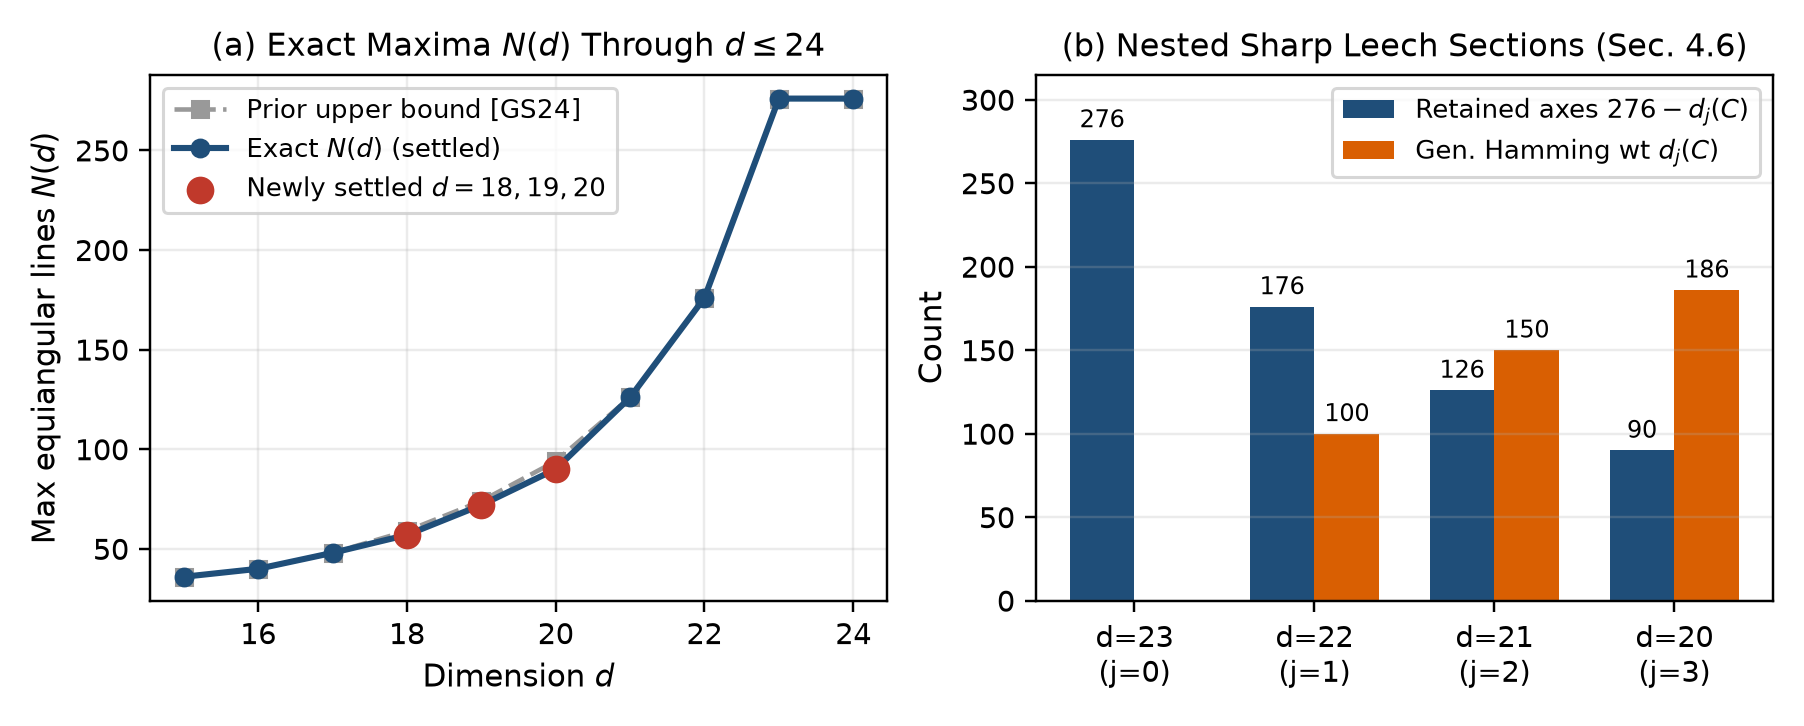
\includegraphics[width=0.96\textwidth]{figures/fig1_maxima_and_leech_sections.png}
\caption{Modes~1--2 certification~\cite{DLY2026}: (a)~settled real equiangular line maxima $N(d)$ through $d \leq 24$ highlighting $N(18)=57, N(19)=72, N(20)=90$ versus prior upper bounds~\cite{GreavesSyatriadi2024}; (b)~exact nested sharp Leech sections $(23,276)\supset(22,176)\supset(21,126)\supset(20,90)$ matching generalized Hamming weights $d_j(C)\in\{100,150,186\}$.}
\label{fig:fig1}
\end{figure*}

\paragraph{Mode 3: Theorem 5.1 Sharp Fixed-Angle Intervals (\texttt{C09}--\texttt{C12}).}
For $k \in \{7, 23\}$ with irrational Bukh--Cox reciprocal bounds $L_7 = 72/(7\sqrt{10}+2)$ and $L_{23} = 600/(23\sqrt{26}+2)$, Mode~3 computes $\lfloor L_k Q \rfloor$ with \emph{zero floating-point operations} by exact integer binary search and squaring, verifies $(t, r, d_-, d_+)$ across the published table instances ($q \in \{19, 111, 321, 5601, 6001\}$; Fig.~\ref{fig:fig2}), and for \texttt{C09} ($q=19, k=7$) explicitly constructs the $56\times 56$, $57\times 57$, and $58\times 58$ Seidel-block extended Gram matrices $\widehat{G}$ of Eq.~(38) and certifies PSD with exact ranks $49, 50, 51$.

\begin{figure*}[tb]
\centering
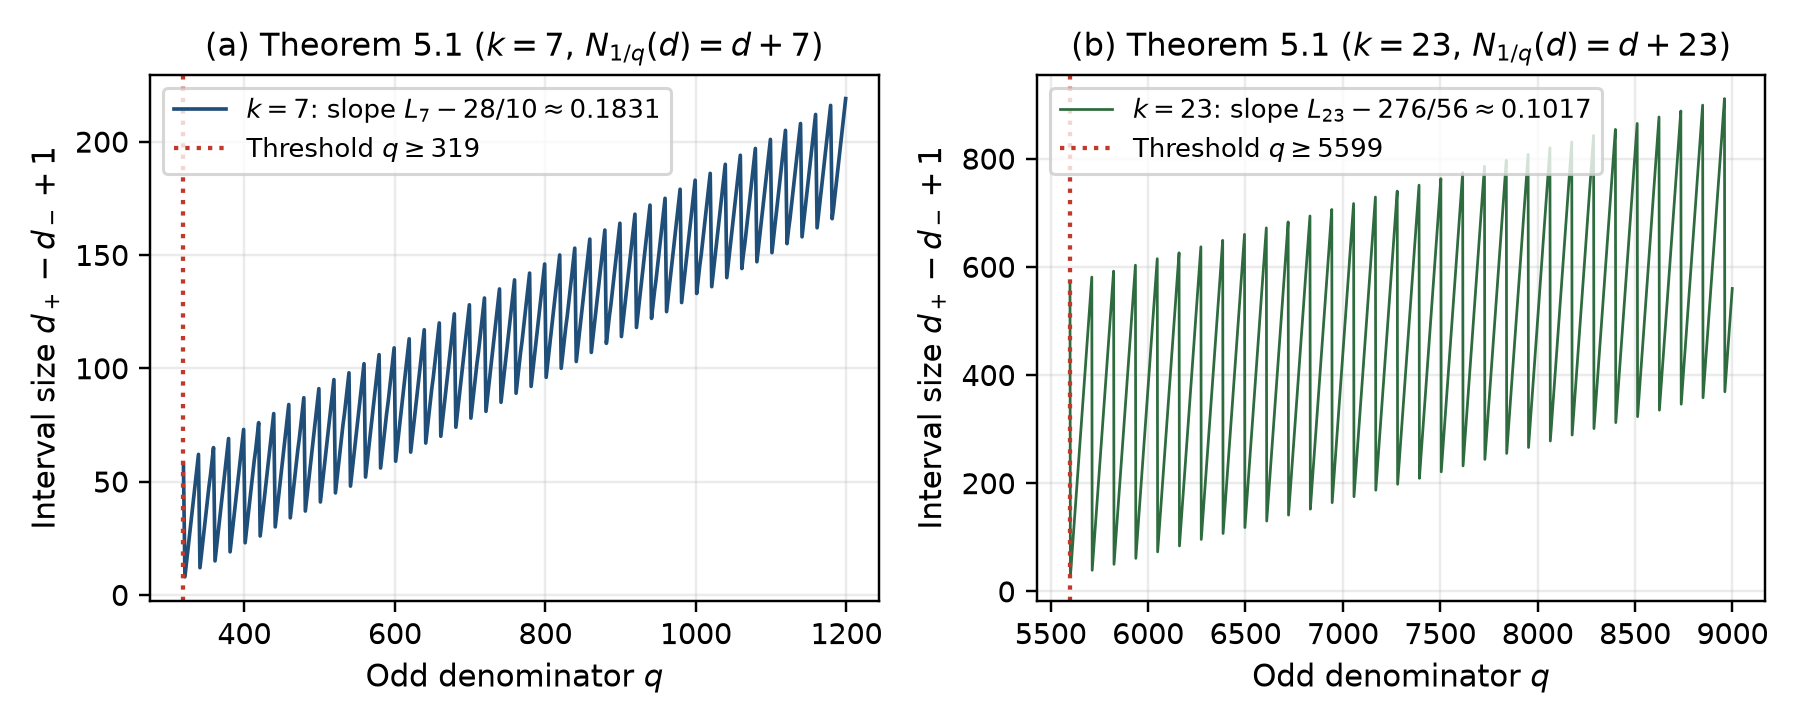
\includegraphics[width=0.96\textwidth]{figures/fig2_fixed_angle_intervals.png}
\caption{Mode~3 certification of Theorem~5.1~\cite{DLY2026}: exact interval widths $d_+ - d_- + 1$ on which $N_{1/q}(d) = d + k$ holds for (a)~$k=7$ above $q \geq 319$ (asymptotic slope $L_7 - 28/10 \approx 0.1831$) and (b)~$k=23$ above $q \geq 5599$ (slope $L_{23} - 276/56 \approx 0.1017$).}
\label{fig:fig2}
\end{figure*}

\paragraph{Mode 4: Paley Conference Matrices \& Cosine $1/7$ (\texttt{C13}--\texttt{C16}).}
Certificates \texttt{C13}--\texttt{C15} construct the exact symmetric Paley conference matrices $C$ of orders $m = p+1$ for $p \in \{5, 13, 17\}$, verify $C^\top = C$, zero diagonal, off-diagonal $\pm 1$, and $C^2 = p I_m$, and verify Theorem~5.2's conjugate-multiplicity trace contradiction certifying $(d, N) = (9,12), (21,28), (27,36)$ at cosine $1/(1+2\sqrt{p})$ (Fig.~\ref{fig:fig3}). Certificate \texttt{C16} (and an additional unit test for $d=10$) constructs Proposition~5.3's explicit scaled Gram matrices $G = 8I_n - 2B + J_n$, where $B = \operatorname{diag}(J_4, J_4, J_4)$ for $n=12$ and $B = \operatorname{diag}(J_4, J_4, J_4, J_1)$ for $n=13$ (with all-ones blocks $J_k$, so $B_{ii} = 1$, diagonal $G_{ii} = 8 - 2 + 1 = 7$, off-diagonal $-1$ inside blocks and $+1$ across blocks, giving common cosine $1/7$), and certifies PSD with exact ranks $10$ and $11$, proving $N_{1/7}(10)=12$ and $N_{1/7}(11)=13$.

\begin{figure*}[tb]
\centering
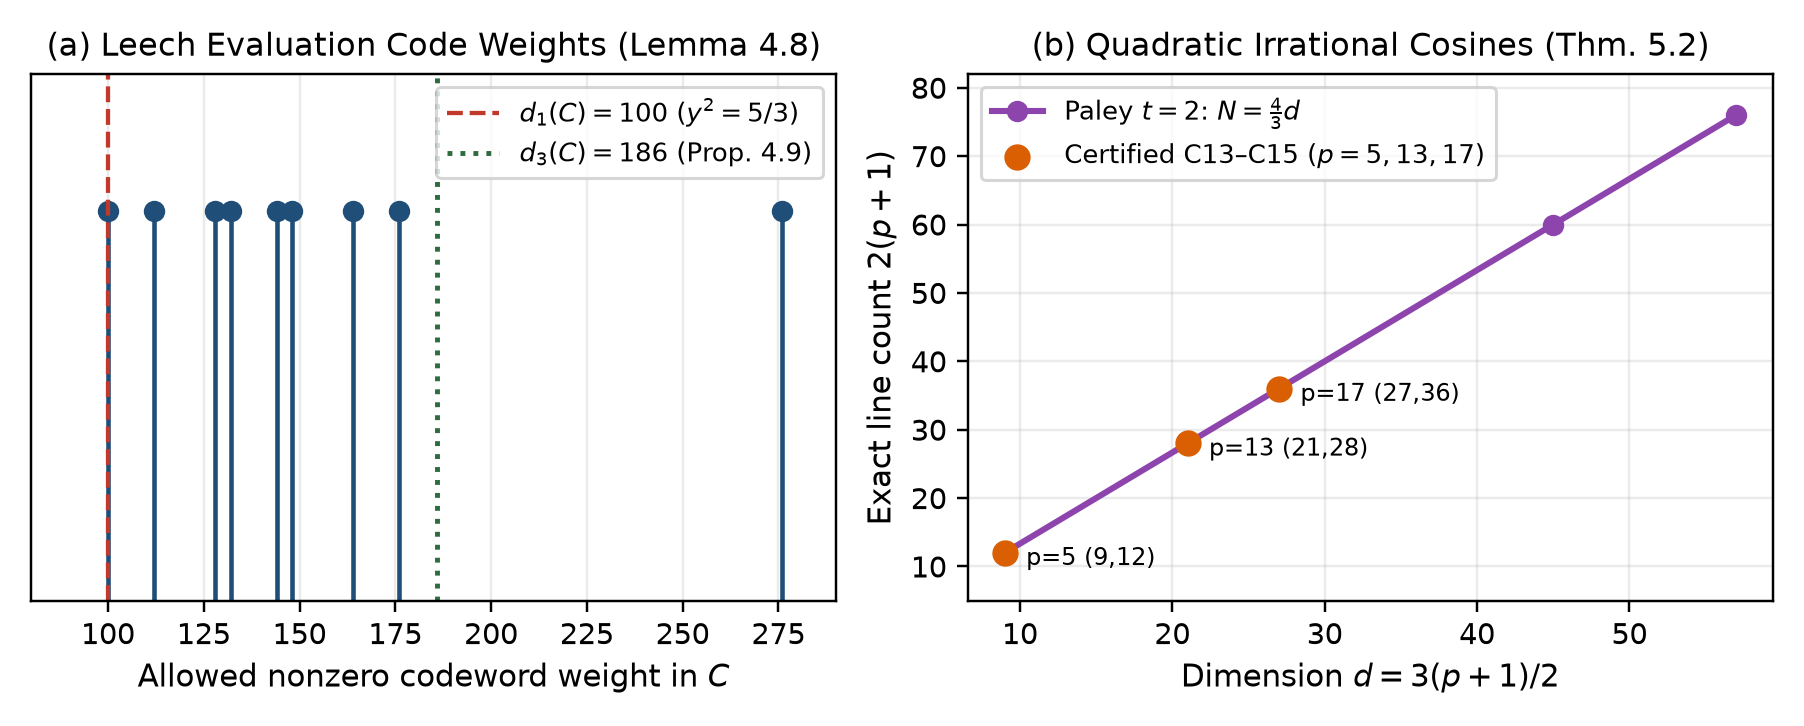
\includegraphics[width=0.96\textwidth]{figures/fig3_golay_weights_and_paley.png}
\caption{Modes~2 and~4 certification~\cite{DLY2026}: (a)~the exact nine allowed nonzero weights of the Leech evaluation code $C$ (Lemma~4.8) with $d_1(C)=100$ and Proposition~4.9's threshold $d_3(C)=186$; (b)~Theorem~5.2's symmetric Paley conference family $N_{1/(1+2\sqrt{p})}(3(p+1)/2) = 2(p+1)$ with certified matrices \texttt{C13}--\texttt{C15}.}
\label{fig:fig3}
\end{figure*}

\section{Verification Results and Forgery Resistance}
All 16 canonical certificates pass verification in $<0.8$\,s (Table~\ref{tab:certs}). The test suite \texttt{tests/test\_verifier.py} runs 32 tests covering all 16 certificates, an AST zero-float audit, Proposition~5.3 at $d=10$, extra Theorem~5.1 table rows ($q=5601, k=7$; $q=6001, k=23$), indefinite-matrix PSD rejection, and 11 targeted forgery attacks (\texttt{32 passed} in $0.77$\,s).

\begin{table*}[tb]
\centering
\caption{Summary of all 16 canonical certificates (\texttt{C01}--\texttt{C16}) verified under \texttt{EQUIANGULAR-D18-20-CERT-1.0}.}
\label{tab:certs}
\scriptsize
\setlength{\tabcolsep}{3pt}
\begin{tabular}{@{}llll@{}}
\toprule
ID & Mode / Submode & Key Parameters & Certified Output / Witness \\
\midrule
\texttt{C01} & \texttt{dim18} (\texttt{prop23\_57\_lines}) & $K_{10}$ matchings + $K_4$ arcs & $57\times 57$ PSD Gram, exact $\operatorname{rank}_{\mathbb{Q}} = 18$ \\
\texttt{C02}--\texttt{C04} & \texttt{dim18} (\texttt{lemma13}) & $(r,\operatorname{rank} T)\in\{(18,2),(19,1),(20,0)\}$ & $w^2=6, x^2=4, (x,w)=3$, rank $\leq 21$ \\
\texttt{C05} & \texttt{leech} (\texttt{golay\_lemma48}) & $G_{24}$ from $X^{11}+X^9+X^7+X^6+X^5+X+1$ & 759 octads, 253 heptads, 9 Lemma~4.8 weights \\
\texttt{C06}--\texttt{C08} & \texttt{leech} (\texttt{nested\_sections}) & $d \in \{22, 21, 20\}$ & PSD Gram ranks $22, 21, 20$; axes $176, 126, 90$ \\
\texttt{C09}--\texttt{C12} & \texttt{fixed\_angle\_thm51} & $(q,k)\in\{(19,7),(111,23),(321,7),(5601,23)\}$ & Exact $[d_-,d_+]$ + $q=19$ Gram ranks $49,50,51$ \\
\texttt{C13}--\texttt{C15} & \texttt{conference} (\texttt{thm52\_paley}) & $p \in \{5, 13, 17\}$, $t = 2$ & Paley $C^2=p I_{p+1}$, $(d,N)=(9,12),(21,28),(27,36)$ \\
\texttt{C16} & \texttt{conference} (\texttt{prop53}) & $d = 11$, $B=\operatorname{diag}(J_4^3,J_1)$ & PSD $G=8I_{13}-2B+J_{13}$ ($G_{ii}=7$), $\operatorname{rank}=11$ \\
\bottomrule
\end{tabular}
\end{table*}

\FloatBarrier
\section{Reproducibility and Transparency}
All code, Lean~4.35.0 proofs, JSON certificates, figures, and \texttt{MANIFEST.sha256} are archived at \url{https://github.com/lluiseriksson/equiangular-lines-dim18-20-certificates} (tag \texttt{v1.0.1}). Independent replay uses Lean~4.35.0 and standard-library Python~$\geq 3.10$:
\begin{quote}\small\raggedright
\texttt{(cd lean \&\& lake build)}\\
\texttt{python -m} \nolinkurl{src.equiangular_dim18_20_verifier} \texttt{certificates}\\
\texttt{pytest -q}
\end{quote}
\noindent\textit{AI Assistance Disclosure:} Formalization, verifier implementation, and manuscript authoring were carried out by Lluis Eriksson using Google Antigravity, with all claims machine-checked by Lean~4.35.0 and the deterministic zero-float verifier. Code/certificates are MIT; manuscript/figures are CC-BY-4.0.

\begin{thebibliography}{9}
\bibitem{DLY2026} V.~Djaljapayan, Z.-Q.~Liao, and W.-H.~Yu, ``Real equiangular lines in dimensions 18--20 and sharp fixed-angle bounds,'' \texttt{arXiv:2611.34855v1} [math.CO], 25 Nov 2026.
\bibitem{LemmensSeidel1973} P.~W.~H.~Lemmens and J.~J.~Seidel, ``Equiangular lines,'' \textit{J.\ Algebra} \textbf{24} (1973) 494--512.
\bibitem{GreavesSyatriadi2024} G.~R.~W.~Greaves and J.~Syatriadi, ``Real equiangular lines in dimension 18 and the Jacobi identity for complementary subgraphs,'' \textit{J.\ Combin.\ Theory Ser.\ A} \textbf{201} (2024) 105812.
\bibitem{BukhCox2020} B.~Bukh and C.~Cox, ``Nearly orthogonal vectors and small antipodal spherical codes,'' \textit{Israel J.\ Math.} \textbf{238} (2020) 359--388.
\bibitem{Lean4} L.~de~Moura and S.~Ullrich, ``The Lean~4 theorem prover and programming language,'' \textit{Proc.\ CADE-28}, LNCS 12699 (2021) 625--635.
\end{thebibliography}

\end{document}
